\documentclass{report}
\usepackage[T1]{fontenc} % Fontes T1
\usepackage[utf8]{inputenc} % Input UTF8
\usepackage[backend=biber, style=ieee]{biblatex} % para usar bibliografia
\usepackage{csquotes}
\usepackage[portuguese]{babel} %Usar língua portuguesa
\usepackage{blindtext} % Gerar texto automaticamente
\usepackage[printonlyused]{acronym}
\usepackage{hyperref} % para autoref
\usepackage{graphicx}
\usepackage{indentfirst}
\usepackage{wrapfig}

\bibliography{bibliografia}


\begin{document}
%%
% Definições
%
\def\titulo{Projeto Final de Laboratórios de Informática}
\def\data{17-06-2023}
\def\autores{Bernardo Marujo, Diogo Carvalho, Rui Rosmaninho, Simão Almeida}
\def\autorescontactos{(107322) bernardomarujo@ua.pt, (113221) diogo.tav.carvalho@ua.pt\\(113553) rui.rosmaninho@ua.pt , (113085) spsa@ua.pt}
\def\departamento{Dept. de Eletrónica, Telecomunicações e Informática}
\def\empresa{Universidade de Aveiro}
\def\logotipo{ua.pdf}
%
%%%%%% CAPA %%%%%%
%
\begin{titlepage}

\begin{center}
%
\vspace*{50mm}
%
{\Huge \titulo}\\ 
%
\vspace{10mm}
%
{\Large \empresa}\\
%
\vspace{10mm}
%
{\LARGE \autores}\\ 
%
\vspace{30mm}
%
\begin{figure}[h]
\center
\includegraphics{\logotipo}
\end{figure}
%
\vspace{30mm}
\end{center}
%
\end{titlepage}

%%  Página de Título %%
\title{%
{\Huge\textbf{\titulo}}\\
{\Large \departamento\\ \empresa}
}
%
\author{%
    \autores \\
    \autorescontactos
}
%
\date{\today}
%
\maketitle

\pagenumbering{roman}

%%%%%% Agradecimentos %%%%%%
% Segundo glisc deveria aparecer após conclusão...
\renewcommand{\abstractname}{Agradecimentos}
\begin{abstract}
O grupo agradece, tanto quanto aos professores que se mostraram presentes e disponíveis a ajudar, tanto aos colegas que se disponibilizaram a ajudar, ao longo do projeto e ao longo do trabalho.
\end{abstract}


\tableofcontents
% \listoftables     % descomentar se necessário
% \listoffigures    % descomentar se necessário


%%%%%%%%%%%%%%%%%%%%%%%%%%%%%%%
\clearpage
\pagenumbering{arabic}

%%%%%%%%%%%%%%%%%%%%%%%%%%%%%%%%
\renewcommand{\abstractname}{Objetivos do projeto}
\begin{abstract}

Neste trabalho foi pedido aos alunos que fizessem uma página com o objetivo de aprender mais sobre as demais tecnologias web, criando uma plataforma de armazenamento e partilha de imagens, de uma forma rápida, e intuitiva. Esta permite os utilizadores criar escrever uma descrição da foto e também comentar e dar \textit{like} e \textit{dislike} as fotos de outros utilizadores. Alem da partilha de imagens, é possível também processá-las.

\end{abstract}

\chapter{Interface}

\label{chap.interface}
\begin{wrapfigure}{l}{0.3\textwidth} % Adjust the width as needed
  \centering
  
\includegraphics[width=0.2\linewidth]{navbar.png}
  \caption{Barra de Navegação}
\end{wrapfigure}

A interface web merece algum destaque, visto que imita a funcionalidade de uma web criada com ajuda de um framework, algo comum hoje em dia, utilizando apenas HTML, CSS e JavaScript, com ajuda do JQuery para manipular alguns elementos na galeria e nos demais sítios em que é exigida a interação entre o CherryPy e a interface. Este método de desenvolvimento, facilita a coerência visual, reduz o código HTML, e melhora a suavidade e performance geral da página.

À esquerda, temos uma barra de navegação, com as opções mais importantes.

\begin{itemize}
    \item Home - O logótipo do website;
    \item Gallery - Contém as imagens guardadas na base de dados;
    \item Process - Página dedicada à manipulação básica de imagem;
    \item About - Contém informações pertinentes ao projeto e aos seus contribuidores;
    \item Upload - Pop-up de upload de imagens;
    \item Logout - Sair da conta, e efetuar login novamente;
    \item Theme - Botão de escolha entre tema de sistema, escuro e claro.
\end{itemize}

\chapter{Armazenamento e manipulação de dados}
\label{chap.dados}

\begin{figure}[htbp]
  \centering
  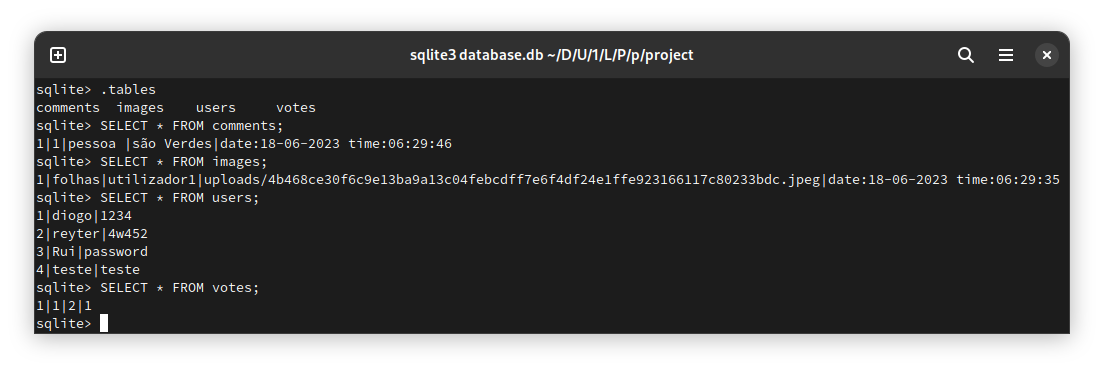
\includegraphics[width=\textwidth]{database.png}
  \caption{Tabela de imagens na base de dados}
  \label{fig:image}
\end{figure}

O projeto em questão apresenta uma sólida infraestrutura, responsável por armazenar e gerir um vasto conjunto de imagens, comentários, e votos. Além de permitir o processamento de imagem na página \textbf{Process}, a base de dados desempenha um papel fundamental ao viabilizar interações mais indiretas entre os usuários, como comentários e votos (positivos ou negativos) sobre as imagens. Essas diversas formas de interação são armazenadas de maneira eficiente, graças à tecnologia SQLite 3.

Graças à robustez desta tecnologia, todas as informações relevantes são registadas de forma segura e estruturada. Através do SQLite, é possível gravar e manipular todos os tipos de dados necessários para o funcionamento adequado do projeto. Além disso, a filtragem dos dados é simplificada, permitindo uma busca mais precisa e rápida de informações específicas.

\chapter{Conclusões}
\label{chap.conclusao}
Apesar das dificuldades encontradas, como a falta de tempo para implementar todas as funcionalidades planeadas e a adaptação a tecnologias novas, o projeto obteve resultados aceitáveis na criação de uma interface web funcional e na implementação de uma base de dados robusta. A interface desenvolvida, que imita a funcionalidade de um framework utilizando apenas tecnologias web tradicionais, proporciona uma experiência coerente, suave e com bom desempenho para os usuários. Já a tecnologia SQLite 3 desempenha um papel fundamental na armazenagem e manipulação dos dados, garantindo segurança e eficiência. Embora nem todas as funcionalidades tenham sido concluídas, o projeto representa o esforço homogéneo no desenvolvimento de uma plataforma que permite o compartilhar e interagir com imagens de uma forma natural e intuitiva.

\chapter*{Contribuições dos autores}
\textbf{Percentagem que cada autor contribuiu.}\\

\autores : 

25\%, 25\%, 25\%, 25\%\\

\textbf{Repositório GitHub:} \href{https://github.com/detiuaveiro/projeto-final-labi2023g7/tree/updated}{labi2023g7}


\end{document}
